\documentclass[a4paper,12pt]{book}
\usepackage{kotex}

\usepackage{amsmath}
\usepackage{amsfonts}
\usepackage{amssymb}
\usepackage[toc,page]{appendix}
\usepackage{array}
\usepackage{atbegshi}
\usepackage{bookmark}
\usepackage{caption}
\usepackage{color}
\usepackage[
    type={CC},
    modifier={by},
    version={4.0},
]{doclicense}
\usepackage{enumitem}
\usepackage{etoolbox}
\usepackage{fancyhdr}
\usepackage{fancyvrb}
\usepackage{float}
\usepackage{graphicx}
\usepackage{hyperref}
\usepackage{hyphenat}
\usepackage{listings}
\usepackage{longtable}
\usepackage[framemethod=tikz]{mdframed}
\usepackage{microtype}
\usepackage{scrlayer}
\usepackage{setspace}
\usepackage{tikz}

\usetikzlibrary{patterns,positioning}

% THEOREM

\newtheorem{exercise}{Exercise}

% MACROS

\newcommand{\cnote}[1]{
    \marginpar{
        \linespread{1}
        \begin{tikzpicture}[pin]
            \foreach \X in {0,...,22} {
                \foreach \Y in {-2,...,2}
                    \filldraw[color=red!45] (\X*2pt+\Y*\Y,-\Y*2pt-4pt) circle ({(5-0.2*\X)*0.1pt});
            }
            \draw (48pt,-4pt) node[right] {\small NOTE};
        \end{tikzpicture}
        \small{#1}
    }
}
\newcommand{\Mod}[1]{\ (\mathrm{mod}\ #1)}
\newcommand{\V}[1]{\Verb|#1|}
\newcommand{\exercise}[1]{
    \begin{exercise} 
        #1 
    \end{exercise}
}

\newcommand{\ccomment}[1]{}

% LSTLISTING

\definecolor{light-gray}{gray}{0.95}
\definecolor{gray}{gray}{0.4}
\lstset{
    columns=fullflexible,
    inputencoding=utf8,
    escapeinside={(*@}{@*)},
    basicstyle=\linespread{1}\small\ttfamily
}
\surroundwithmdframed[
  hidealllines=true,
  backgroundcolor=light-gray,
  innerleftmargin=15pt,
  innertopmargin=0pt,
  innerbottommargin=0pt]{lstlisting}

% STYLES

\AtBeginEnvironment{quote}{\par\singlespacing}

\setlist[enumerate]{noitemsep}
\setlist[itemize]{noitemsep}
\AtBeginEnvironment{enumerate}{\linespread{1}}

%================================%
% DOCUMENT                       %
%================================%

\title{Introduction to C Programming Language}
\author{서영원}
\date{April 2024}
\begin{document}

\linespread{1.5}

\maketitle

\tableofcontents

\vfill
\doclicenseThis


\pagebreak

\microtypesetup{activate=false}

%================================%

\chapter{들어가기에 앞서}

%================================%

\section{작가의 말}

본 도서는 독자가 고1 수준 수학의 개념을 모두 알고 있다는 전제 하에 서술되었다.
혹여나 모른다고해서 걱정하지 말라, 모두 쉽게 풀어 설명되어있다.

글을 읽다보면 이곳 저곳에 개념의 역사 등 자잘한 것들을 서술하는 방주(旁註)가 작성되어있다.
딱히 읽어야만 하는 것은 아니지만, 교양과목을 듣는다는 마음으로 찬찬히 읽어보도록 하자.

%================================%

\section{사전 준비}

\textit{제작 플랫폼 간단 소개 (회원가입 등)}

%================================%

\chapter{C언어 소개}

%================================%

\section{C언어의 탄생}

운영체제와 브라우저, 온갖 응용프로그램들까지 현대에 이르러 더이상
C언어의 손길을 거치지 않은 프로그램은 없다.
컴퓨터는 인간이 이해할 수 있는 언어는 이해하지 못한다고들 하는데,
그렇다면 C언어는 어떻게 컴퓨터 시스템에서 실행될 수 있을까?
인간이 지금껏 사용해온 언어, 자연어는 왜 컴퓨터 시스템에서 사용되지 않는
것일까?

%================================%

\subsection{자연어의 모호성}

\begin{quote}
`마트가서 우유사고 만약에 아보카도 있으면 6개 사와'
\end{quote}

오늘 독자가 아내로부터 하달받은 명령이다.
우리는 이를 해석함에 있어서 다음과 같이 2가지 해석을 마련할 수 있다.

\begin{center}

    \centering

    아보카도 명령 코드

    \begin{minipage}{0.45\textwidth}
        \begin{lstlisting}[escapeinside=``]
`마트로 이동한다.`
`우유 1개 구매한다.`
`만약 아보카도가 진열되어있다면:`
    `아보카도 6개 구매한다.`
        \end{lstlisting}
    \end{minipage}
    \hfill
    \begin{minipage}{0.45\textwidth}
        \begin{lstlisting}[escapeinside=``]
`마트로 이동한다.`
`만약 아보카도가 진열되어있다면:`
    `우유 6개 구매한다.`
`아니라면:`
    `우유 1개 구매한다.`
        \end{lstlisting}
    \end{minipage}

\end{center}

만에 하나 둘 중에 잘못된 선택지를 골랐다면 (우유 6팩을 구매한다는 둥)
감히 끔찍한 일이 닥치고 말 것이다.

마찬가지로, 컴퓨터를 프로그램함\footnote{프로그램을 컴퓨터에 내장하는 \\
행위}에 있어서 이러한 모호성이 존재할 경우 이가 실행될 때에 컴퓨터는 둘
중 어떠한 행위를 해야할 지 선택해야만 한다. 이는 사용자가 의도하지 않은
동작을 초래할 수 있는 매우 위험한 상태다. 따라서, 그 자체로 모호성을
내재한 자연어는 컴퓨터를 프로그램하기 위한 언어로 적절하지 못하다.

%================================%

\subsection{명령집합과 기계어}

\begin{table}[!h]
    \centering

    \caption{아보카도 명령 집합}
    \label{Tab:avocado-isa}

    \begin{tabular}{ || m{2em} | m{3.8em} | m{22em} || }
        \hline
        이름 & 매개변수 & 동작 \\
        \hline\hline
        buy & 물품 t, 자연수 n & t를 n개 만큼 구매한다. 아니라면 0으로 정의한다 \\
        \hline
        find & 물품 t & 물품 t가 존재한다면 r을 1로 정의한다. 아니라면 r을 0으로 정의한다. \\
        \hline
        move & 위치 p & r이 0이라면 위치 p로 이동한다. 아니라면 아무 동작도 하지 않는다. \\
        \hline
    \end{tabular}
    \newline
    \textit{\color{gray} \small r은 미지수 내지 변수라고 정의하자.
    아직 너무 엄밀해질 필요는 없다.}
\end{table}

대신, 컴퓨터는 인위적으로 정의된 명령 집합에 따라 작동한다. 아보카도와
우유를 향한 임무 달성을 위해 Table \ref{Tab:avocado-isa} 과 같이 명령
집합을 정의해보자.

이러한 명령집합을 사용하면 아래와 같이 \textbf{엄밀하게} 우리의 행위를
정의해볼 수 있다. (명령은 위에서부터 순차적으로 실행한다.)

\begin{center}

    \centering

    아보카도 명령 코드 (최종)

    \begin{minipage}{0.45\textwidth}
        \begin{lstlisting}[escapeinside=``]
buy(`우유`, 1)
find(`아보카도`)
move(`출구`)
buy(`아보카도`, 6)
        \end{lstlisting}
    \end{minipage}
    \hfill
    \begin{minipage}{0.45\textwidth}
        \begin{lstlisting}[escapeinside=``]
buy(`우유`, 1)
find(`아보카도`)
move(`출구`)
buy(`우유`, 5)
        \end{lstlisting}
    \end{minipage}

\end{center}

이렇게만 적어도 사람이 프로그램을 수행함에 있어서 어려움은 없다.
그러나, 전류 흐름의 여부로 신호를 처리하는 컴퓨터에게 있어서,
한글과 알파벳을 이해하도록 하는 것은 매우 복잡할 것이다.
% (컴퓨터가 어떻게 글자를 처리하는 지에 대해선 뒤 \autoref{sec:code-page}와 \autoref{sec:fonts}를 참조하라)

따라서, 우리는 다음과 같이 각각의 명령과 단어들에 번호를 부여할 것이다.

\begin{table}[!h]
    \centering

    \caption{아보카도 명령 집합 (최종)}
    \label{Tab:avocado-isa-int}

    \begin{tabular}{ || c | c | c | c || }
        \hline
        이름 & 번호 & 이름     & 번호 \\
        \hline\hline
        buy  & 0    & 아보카도 & 0    \\
        \hline
        find & 1    & 우유     & 1    \\
        \hline
        move & 2    & 출구     & 2    \\
        \hline
    \end{tabular}
\end{table}

부여된 번호를 통해 다시 구현하면 다음과 같다.

\begin{center}

    \centering

    아보카도 명령 코드 (진짜최종)

    \begin{minipage}{0.45\textwidth}
        \begin{lstlisting}
0(1, 1)
1(0)
2(2)
0(0, 6)
        \end{lstlisting}
    \end{minipage}
    \hfill
    \begin{minipage}{0.45\textwidth}
        \begin{lstlisting}
0(1, 1)
1(0)
2(2)
0(1, 5)
        \end{lstlisting}
    \end{minipage}

\end{center}

또한 다음의 규칙에 따라 명령을 기계가 이해하기 쉽도록 바꾸어보자.

\begin{itemize}
    \item 명령과 상품에는 각각 2비트를 할당하자
    \item 상품의 갯수에는 4비트를 할당하자
\end{itemize}

결과는 다음과 같다:

\begin{center}

    \centering
    
    아보카도 명령 코드 (진짜최종2)

    \begin{minipage}{0.45\textwidth}
        \begin{lstlisting}
00 01 0001
01 00
10 10
00 00 0110
        \end{lstlisting}
    \end{minipage}
    \hfill
    \begin{minipage}{0.45\textwidth}
        \begin{lstlisting}
00 01 0001
01 00
10 10
00 01 0101
        \end{lstlisting}
    \end{minipage}

\end{center}

축하한다! 독자는 방금 마트에 가서 우유 (혹은 아보카도)를 구매할
로봇가정부를 위한 명령 체계\footnote{Instruction Set Architecture를 줄여 ISA라고도 부른다.}를 완성했다!
이제 독자는 독자의 아내에게 \textbf{모호하지 않은} 명령을 내려달라고
요구할 수 있게 되었고, 독자의 아내가 독자에게 부여한 업무를 독자의
로봇에게 \textbf{모호함} 없이 전달할 수 있을 것이다!

%================================%

\subsection{기계어와 C언어}

\cnote{
    어셈블리어는 Maurice Wilkes, David Wheeler와 Stanley Gill의 저서
    \textit{The Preparation of Programs for an Electronic Digital Computer}
    에서 최초로 제시되었다.
    본 도서에는 이 외에 최초로 \textit{재사용 가능한} 코드, \textit{API},
    디버깅을 위해 \textit{메모리 덤프}를 사용하는 방법이 서술되었다.
}

...그래서 이 기계어가 C언어랑 무슨 상관일까?
그것은 C언어의 태생에 있다.
자세히 알아보기 위해 1951년으로 돌아가보자.

%================================%

\subsubsection{복잡해지는 ISA와 어셈블리어}

| 컴퓨터를 프로그램하기 위해 0과 1만 두드리고 있는 것은
매우 지루한 일일 뿐더러, 코드에 오류가 존재하거나 오타를 치고 말았을때
수정하기 매우 번거롭다.

개발자들은 이러한 문제를 해결하기 위해
\textit{어셈블리어}\footnote{ASseMbly language를 줄여 ASM이라고 부른다.}를 도입했다. 


이는 독자가 설계한 `아보카도 명령 코드 (최종)'과 비슷한 것으로,
기계어에 일대일 대응되도록 알파벳으로 이루어진 이름을 부여한 것이다.

다음의 규칙과 함께 아래의 명령을 해석해보자:

\begin{table}[!h]
    \centering

    \caption{계산기 ISA}
    \label{Tab:simple-calculator-isa}

    \begin{tabular}{ || m{2em} | m{5em} | m{22em} || }
        \hline
        이름 & 매개변수 & 동작 \\
        \hline\hline
        add  & 값 t & 변수 a에 t만큼 더한 값을 a로 정의한다 \\
        \hline
        mul  & 값 t & 변수 a와 t를 곱한 값을 a로 정의한다 \\
        \hline
        div  & 값 t & 변수 a를 t로 나눈 값을 a로 정의한다 \\
        \hline
        mov  & 변수 a, 값 v & a에 v를 대입한다 \\
        \hline
    \end{tabular}
\end{table}

\begin{center}

    \centering
    
    Table \ref{Tab:simple-calculator-isa}를 이용한 코드

\begin{lstlisting}
mov b, a
add 1
mul b
div 2
mov b, a
\end{lstlisting}
\end{center}

위의 코드는 정의된 ISA에 따라 아래와 같은 수식으로 해석할 수 있다:

\begin{equation}
b = \frac{a(a + 1)}{2}
\end{equation}

하지만, 세상에 이렇게 간단한 코드만 존재했다면 세상은 지금까지조차 ASM을
쓰고 있을지도 모르겠다.
그럼 그렇지, 요즘 많이 사용되는 x86-64 구조는 명령어 약 3,600개 가량을
가지고 있다.
이 것들을 아무런 도움도 없이 활용하여 성능 좋고 보기도 좋은 프로그램을
만드는 것은 매우 어려운 일이다.

%================================%

\subsubsection{고수준 언어의 등장}

| 개발자들은 \textbf{사람이 이해하기 쉬운} 프로그래밍 언어를 원했다.
결국 1953년, IBM의 John Backus는 세계 최초의 고수준 프로그래밍 언어,
\textit{Speedcoding}을 개발했다.

\begin{figure}[!h]
    \centering
    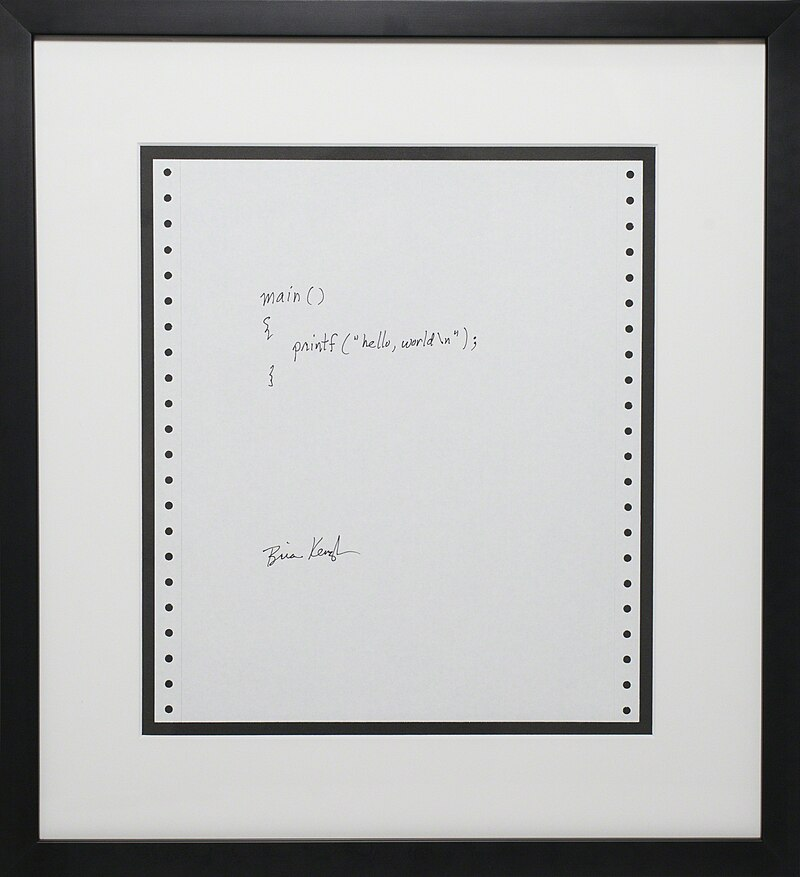
\includegraphics[width=\linewidth]{images/hello-world.jpg}
    \caption{1978년, C언어를 공동개발한 Brian Kernighan의 Hello, World}
\end{figure}

이후 \textit{Fortran}(1957), \textit{ALGOL}(1960), \textit{CPL}(1963)과
\textit{B}(1969)를 거치고, 드디어 1972년 벨 연구소, Dennis Ritchie는
\textit{C}를 개발한다.

\pagebreak

%================================%

\section{Hello, World!}

C언어는 기본적으로 ASM과 같은 저급언어을 추상화하기 위해 태어난 여러 언어들의 문제점들을 해결하기 위해 만들어졌다.
따라서, C언어의 문법을 이해하기 위해, 먼저 초보자를 위해 설계된 BASIC으로 작성된 예제를 살펴보자.

(본 단원은 반복문, 함수의 개념을 언어의 발전과정을 통해 이해하기 쉽게 하기 위한 단원이다.
이미 반복문, 조건문, 함수의 개념을 알고있다면, 곧바로 \autoref{sec:hello-c}로 넘어가도 좋다!)

%================================%

\subsection{Hello, BASIC!}

\begin{lstlisting}
10 PRINT "Hello, BASIC!"
20 END
\end{lstlisting}

위는 BASIC을 통해 화면에 `Hello, BASIC!'라는 문장을 출력하는 예제다.

영어를 할줄 안다면 대충 이해했을텐데, 
첫 줄의 \V{PRINT ``Hello, BASIC!"}는 `Hello, BASIC!'라는 문장을 출력하도록 하는 명령,
두번째 줄의 `END'는 프로그램이 종료되었음을 알리는 명령이다.

\exercise{위 코드를 직접 실행해보자!}
\exercise{\V{Hello, BASIC!}대신에 다른 문장을 넣어보고, 어떻게 되는지 확인해보자!}

%================================%

\subsection{더 깊은 곳으로}

더 복잡한 예시를 살펴보자.

\begin{lstlisting}
10 N=100
20 FOR I=1 TO N
30 PRINT "Hello, BASIC!"
40 NEXT I
\end{lstlisting}

위의 예시는 다음의 과정에 따라 \V{Hello, BASIC!}라는 문장을 100번 출력하는 예제다:

첫 줄의 명령:

\begin{lstlisting}
10 N=100
\end{lstlisting}

는 변수 \V{N}의 값을 100으로 정의한다.

\begin{lstlisting}
20 FOR I=1 TO n
...
40 NEXT I
\end{lstlisting}

에서, \V{FOR I=1 TO N}은 변수 I이 1에서 N까지 이산적으로 증가
($\textstyle \sum\limits_{I=1}^N$)하는 동안,
`\V{...}'에 있는 명령들을 실행하도록 한다.
이렇게, 어떤 명령들을 쉽게 반복할 수 있게 해주는 구문을 `반복문(loop)'이라고 한다.

다음 줄의 구문:

\begin{lstlisting}
30 PRINT "Hello, BASIC!"
\end{lstlisting}

은 \V{Hello, BASIC!}이라는 문장을 출력한다.

\exercise{N과 I의 값을 변경하고, 출력이 어떻게 변화하는지 살펴보자!}

%================================%

\subsection{입력 받기}

BASIC에서 출력 뿐만 아니라, 입력을 받아볼 수도 있지 않을까?
다음의 예시를 살펴보자:

\begin{lstlisting}
10 INPUT "How many stars? "; C
20 S$ = ""
30 FOR I=1 TO C
40 S$ = S$ + "*"
50 NEXT I
60 PRINT S$
70 INPUT "Do you want more? "; A$
80 IF LEN(A$) = 0 THEN GOTO 70
90 IF A$ = "y" OR A$ = "Y" THEN GOTO 10
100 PRINT "Goodbye"
110 END
\end{lstlisting}

\begin{lstlisting}
10 INPUT "How many stars? "; C
\end{lstlisting}

는 `\V{How many stars? }'를 출력하고, 입력값을 변수 C에 저장한다.

\begin{lstlisting}
20 S$ = ""
\end{lstlisting}

는 변수 \V{S\$}의 값을 빈 문자열 \V{``''}로 정의한다.

\begin{lstlisting}
30 FOR I=1 TO C
40 S$ = S$ + "*"
50 NEXT I
\end{lstlisting}

는 변수 \V{I}의 값을 1에서 \V{C}까지 변화시키며,
변수 \V{S\$}의 뒤에 \V{*}를 한글자씩 덧붙인다.

\begin{lstlisting}
60 PRINT S$
\end{lstlisting}

는 현재 \V{S\$}의 값을 출력한다.

\begin{lstlisting}
70 INPUT "Do you want more? "; A$
\end{lstlisting}

는 `\V{Do you want more? }'을 출력하고,
입력값을 변수 \V{A\$}에 저장한다.

\begin{lstlisting}
80 IF LEN(A$) = 0 THEN GOTO 70
\end{lstlisting}

위 구문은 아래와 같이 해석할 수 있다:

\begin{itemize}
    \item `\V{IF ... THEN ...}'는 \V{IF}뒤의 조건이 만족되었을때,
    \V{THEN}뒤의 명령을 수행한다.
    이렇게 조건에 따라 명령의 수행 여부를 결정하는 구문을 `조건문'이라고 한다.
    \item \V{LEN(A\$)}는 변수 `\V{A\$}'의 길이(글자의 개수)를 의미한다.
    \item `\V{GOTO 70}'은 70번째 줄(명령 앞에 붙은 번호)로 이동하라는 의미이다.
\end{itemize}

따라서, 입력(\V{A\$})의 글자수가 0이라면, 70번째 줄로 이동하라는 의미이다.

\begin{lstlisting}
90 IF A$ = "y" OR A$ = "Y" THEN GOTO 10
\end{lstlisting}

는 입력(\V{A\$})가 \V{y} 또는(\V{OR}) \V{Y}라면, 10번째 줄로 이동하라는 의미이다.

\begin{lstlisting}
100 PRINT "Goodbye"
110 END
\end{lstlisting}

는 \V{Goodbye}를 출력하고, 프로그램을 종료하라는 의미이다.

결국, 위 프로그램은 입력받은 숫자만큼 `*'을 출력하는 프로그램이다.
프로그래밍에 익숙하지 않거나, `goto'를 사용해본적 없다면, 위 코드부터 슬슬 어지러움을 느낄 수 있다.
물론, 아직까지 어지럼증을 느끼지 않을 순 있으나, `*'와 `-' 중 선택한 문자를 출력하도록 하는 프로그램이라던지,
여러 기능들을 추가하다보면 점점 내가 뭘 하고있는지 알수 없게되는 시점이 온다.

이를 해결하기 위해 개발자들은 언어를 `구조화'시키기 시작했다.

%================================%

\subsection{Label과 Goto}

개발자는 먼저 줄번호(명령의 앞에 붙어 명령의 번호와 순서를 지정하는 번호)를 없애고, 대신 `레이블(label)'을 도입했다.
예를 들면 다음과 같다:

\begin{center}

    \centering
    
    줄번호를 이용한 BASIC(좌)과 label을 이용한 BASIC(우)

    \begin{minipage}{0.45\textwidth}
        \begin{lstlisting}
10 PRINT "Hello!"
20 GOTO 10
        \end{lstlisting}
    \end{minipage}
    \hfill
    \begin{minipage}{0.45\textwidth}
        \begin{lstlisting}
Print:
PRINT "Hello!"
GOTO Print
        \end{lstlisting}
    \end{minipage}

\end{center}

\cnote{
    Syntax Sugar:
    없으면 프로그램을 구현하지 못하는게 아닌데도, 사람이 표현하기 쉽도록 설계된 문법.
}

훨씬 가독성이 좋아진 모습이나,
`GOTO'가 코드에 보이는 것 조차 싫었던 개발자들은 `GOTO'없이 코드를 작성하기 위해 여러 문법 설탕들과 `서브루틴(subroutine)'의 개념을 추가했다.

%================================%

\subsection{DO WHILE ... LOOP}

2세대 BASIC언어들에는 참 많은 문법 설탕들이 있지만,
그중에서도 `DO WHILE ... LOOP'를 소개하고자 한다.

\begin{center}
    \centering

    `\V{GOTO}'(상)와 `\V{DO WHILE ... LOOP}'(하)

\begin{lstlisting}
Print:
PRINT "Hello, BASIC!"
INPUT "Want one more line? "; S$
IF S$ = "y" OR S$ = "Y" THEN GOTO Print
\end{lstlisting}
\begin{lstlisting}
PRINT "Hello, BASIC!"
INPUT "Want one more line? "; S$
DO WHILE S$ = "y" OR S$ = "Y"
    PRINT "Hello, BASIC!"
    INPUT "Want one more line? "; S$
LOOP
\end{lstlisting}

\end{center}

label을 없애고 WHILE을 통해 직관적으로 반복문의 구조와 조건을 밝히며 가독성을 높이고 있다.
그러나, 같은 명령이 두번씩 반복되는 것은 그다지 좋지 않은 코드다.
%(`그다지 좋지 못한 코드'가 무엇인지 궁금한 독자는 \autoref{sec:clean-code}를 참조하라.)
이런 상황을 위해 `DO ... LOOP WHILE'문이 준비되어있다.



\begin{center}
    \centering

    `\V{DO WHILE ... LOOP}'(상)와 `\V{DO ... LOOP WHILE}'(하)

\begin{lstlisting}
PRINT "Hello, BASIC!"
INPUT "Want one more line? "; S$
DO WHILE S$ = "y" OR S$ = "Y"
    PRINT "Hello, BASIC!"
    INPUT "Want one more line? "; S$
LOOP
\end{lstlisting}
\begin{lstlisting}
S$ = ""
DO
    PRINT "Hello, BASIC!"
    INPUT "Want one more line? "; S$
LOOP WHILE S$ = "y" OR S$ = "Y"
\end{lstlisting}

\end{center}

반복문 내의 코드를 실행하기 이전에 조건을 검사해, 두번씩 작성되던 코드를 한번만 작성할 수 있게 했다.

이와 같이 BASIC과 많은 언어들은 문법 설탕을 첨가하며 발전해왔고, C언어 또한 이러한 구조들을 채택하고 있다.
이제 서브루틴에 대해 알아보자.

%================================%

\subsection{서브루틴}

특정한 갯수 만큼 별표(`*')를 출력하는 등 자주 반복되는 명령들을 하나로 묶어서 사용할 순 없을까?
묶어서 사용할 수만 있으면, 같은 명령어들이 반복해서 쓰이는 상황들도 효과적으로 줄일 수 있을 것이다.

이러한 고민 속에 탄생한 것이 서브루틴으로,
단순히 말하자면, 특정한 일을 처리하기 위해 일련의 명령어들을 묶어둔 것이다.

쉬운 이해를 위해 BASIC코드를 보며 이해해보자:

\begin{lstlisting}
10 GOSUB 100
20 PRINT "Bye, SUBROUTINE!"
30 END
100 PRINT "Hello, SUBROUTINE!"
110 RETURN
\end{lstlisting}

위 코드에서 `GOSUB 100'은 `GOTO'와 같이 줄번호 100으로 점프하고,
`PRINT ``Hello, SUBROUTINE!"'과 `RETURN'을 순차적으로 실행시킨다.
유일한 차이점은, `RETURN'이 실행되면 줄번호 10의 자리로 돌아와
'PRINT ``Bye, SUBROUTINE!"을 실행한다는 것이다.

이와 같이 서브루틴은 특정한 주소 공간에 명령어를 모아서 작성할 수 있게 하고,
이를 통해 코드의 유지보수를 쉽게 만들어준다.

그러나, 기술이 발전하고 BASIC에서 줄번호를 없애는 과정속에서 `GOSUB' 또한 개량되어야 했다.
이를 해결하기 위해 개발자들은 `함수(function)'이라는 개념을 도입했다.

%================================%

\subsection{함수}

독자가 한국인이라면, 함수는 중학교에서 알게된 수학 용어일 것이다.
프로그래밍에서의 `함수'또한 비슷한 의미로,
입력을 받아 (정의역에 대해) 일을 처리하기 위해 (출력을 가지기 위해; 치역을 가지기 위해)
묶어놓은 일련의 명령어 묶음이다. (물론, 입력을 받지 않아도 좋다. 이에 대해선 후술한다.)

BASIC에서는 함수를 다음과 같이 작성한다:

\begin{lstlisting}[escapeinside=``]
SUB `함수명`(`매개변수1`, `매개변수2`, ...)
    `명령어...`
END SUB
\end{lstlisting}

위에서 `GOSUB'와 함께 서술된 코드를 함수 문법을 통해 다시 작성해보자:

\begin{lstlisting}
CALL PrintHello()
PRINT "Bye, SUBROUTINE!"
END

SUB PrintHello()
    PRINT "Hello, SUBROUTINE!"
END SUB
\end{lstlisting}

위와 같이, 그저 반복되는 명령어들을 하나로 함축하기 위함이라면 매개변수,
즉 입력을 받지 않아도 좋다.

%================================%

\subsection{Hello, C!}
\label{sec:hello-c}

C언어는 상술된 개념들을 대부분 문법적인 개량만 가지고 차용하고 있다.
이제 C언어를 통해 `Hello, World!'를 출력해보자!


\begin{lstlisting}
main()
{
    printf("Hello, World!\n");
}
\end{lstlisting}

위 C언어 코드는 아래의 BASIC 코드와 동일하다:

\begin{lstlisting}
CALL main()

SUB main()
    PRINT "Hello, World!"
END SUB
\end{lstlisting}

C언어에서는 함수를 정의하는데에 있어서,
서브루틴이라는 개념보다 본격적으로 수학에서의 함수를 닮았다.

수학에서 함수를 $f(x) = ...$와 같이 서술했던 것과 비슷하게,
C언어에서도 함수를 \V{f(x) \{ ... \}}라고 작성한다.
물론, 입력을 받지 않고 단순하게 \V{f()}라고도 작성할 수 있다.

비슷한 맥락에서, \V{main()}은 매개변수를 가지지 않는 `main'이라는 이름의 함수를 선언한 것이고,
그 밑의 \V{\{ ... \}}는 이 함수가 어떤 일을 하는지 서술한다.

따라서, 위의 C언어 코드의 \V{main()}은 호출되었을때,
`\V{Hello, World!\textbackslash{}n}'
(\textbackslash{}n는 개행을 표현하기 위한 특수문자다.
자세한 내용은 \autoref{sec:escapes}를 참조하라.)
를 출력하는 함수라고 말할 수 있다.

또한, BASIC에서만 볼 수 있는 첫 행의 `CALL main()'은 왜 추가된 것일까?
사실, C언어에서는 BASIC처럼 함수에 포함되지 않는 명령을 작성할 수 없다.
글로 읽어서는 이해하기 힘든데, 다음의 코드를 보며 이해해보자:

\begin{center}

    \centering
    
    문법적인 오류가 있는 코드 전문(좌)와 올바른 코드 전문(우)

    \begin{minipage}{0.45\textwidth}
        \begin{lstlisting}
printf("Hello, World!");
printf("Bye...");
        \end{lstlisting}
    \end{minipage}
    \hfill
    \begin{minipage}{0.45\textwidth}
        \begin{lstlisting}
main()
{
    printf("Hello, World!");
    printf("Bye...");
}
        \end{lstlisting}
    \end{minipage}

\end{center}

위와 같이, 모든 명령은 함수 내부에 있어야 한다.

또한, 유독 \V{main()}이라는 이름이 많이 보이는 것 같다면 착각이 아니다.
프로그램의 진입점, 즉 프로그램이 시작하는 부분을 BASIC에서는 위에서부터
순차적으로 실행했다면, C언어에서는 \V{main()}라는 함수를 진입점으로 사용하여,
\V{main()} 함수 내부의 명령부터 실행하게 된다.

%================================%

\subsubsection{세미콜론;;;}

C 코드를 보다보면, 눈에 띄는 기호 하나가 보인다.
바로 세미콜론(;)인데, BASIC에서 명령과 명령을 개행으로 구분했다면,
C언어에서는 이 세미콜론으로 명령을 구분하기 때문에,
모든 명령의 끝에는 세미콜론이 자리잡고 있다.

%================================%

\section{변수와 산술}

\begin{lstlisting}
1 1
2 4
3 9
4 16
5 25
6 36
7 49
8 64
9 81
\end{lstlisting}

위와 같이, 어떤 자연수와 그 제곱을 출력하는 프로그램을 작성해보자!
아래는 위의 출력을 가지는 C 프로그램이다.
프로그램을 하나하나 분석해보자:

\begin{lstlisting}
main()
{
    int integer = 1, square;

    while (integer <= 9)
    {
        square = integer * integer;
        printf("%d %d\n", integer, square);
        integer = integer + 1;
    }
}
\end{lstlisting}

C언어에서 모든 변수는 사용되기 전에 선언(declare)되어야한다.
변수 선언(declaration)은 형식과 변수명으로 이루어진다.
예를 들어:

\begin{lstlisting}
int integer = 1, square;
\end{lstlisting}

는 변수 \V{integer}와 \V{square}의 형식이 \V{int}임을 선언하며,
\V{integer}의 값을 1로 정의한다.
수학 교재 등지에서 변수를 사용할때,
`정수 $a$에 대해' 혹은 `$a \in \mathbb{Z}$' 등의 표기를 본 적 있을 것이다.
마찬가지로, C언어에서도 변수명과 함께 변수의 형식을 병기한다.

\V{int}는 영단어 integer의 약어로서 정수 형식을 표현하는 것으로,
\V{int}외에도 C언어에는 형식을 지정하기위한 여러 키워드들이 예약되어있다:

\begin{table}[H]
    \centering

    \caption{C언어의 기본 산술 형식(basic arithmetic types)}
    \label{Tab:basic-arithmetic-types}

    \begin{tabular}{ || m{4em} | m{26em} || }
        \hline
        형식    & 설명 \\
        \hline\hline
        char   & 기기에서 기본 글자를 표현하기 위한 최소 단위로서, 정수다; 보통 8bit를 가진다 \\
        \hline
        int    & 정수; 보통 32bit를 가진다 \\
        \hline
        float  & 부동소수점(floating-point number) 형식; 보통 IEEE754 단정도 부동소수점 형식(32bit)을 따른다 \\
        \hline
        double & 부동소수점(floating-point number) 형식; 보통 IEEE754 배정도 부동소수점 형식(64bit)을 따른다 \\
        \hline
    \end{tabular}
    \newline
    \textit{\color{gray} \small `bit'가 무엇인지 모르는 독자에겐
    \autoref{sec:digit-oper}가 도움이 될 것이다!}
\end{table}

이러한 형식들은 다음의 수식자(modifier)에 의해 수식될 수 있다:

\begin{table}[H]
    \centering

    \caption{C언어의 형식 수식자(modifier)}
    \label{Tab:type-modifier}

    \begin{tabular}{ || m{4em} | m{9.9em} || m{4em} | m{9.9em} || }
        \hline
        형식 & 설명 & 형식 & 설명\\
        \hline\hline
        long & 형식을 확장한다 & short & 형식을 축소한다 \\
        \hline
        signed & 형식을 부호있는 형식으로 명시한다 & unsigned & 형식을 부호없는 형식으로 명시한다 \\
        \hline
    \end{tabular}
\end{table}

기본 산술 형식과 수식자를 조합해, 다음의 원시 형식(primitive types)들을 조합해낼 수 있다:

\begin{table}[H]
    \centering

    \caption{C언어의 원시 형식(primitive types)}
    \label{Tab:primitive-types}

    \begin{tabular}{ || m{6em} | m{24em} || }
        \hline
        형식           & 설명 \\
        \hline\hline
        char          & 기기에서 기본 글자를 표현하기 위한 최소 단위로서, 정수다; 보통 8bit를 가진다 \\
        \hline
        \hline
        short int     & 짧은 정수 형식; 보통 16bit를 가진다 \\
        \hline
        int           & 정수 형식; 보통 32bit를 가진다 \\
        \hline
        long int      & 긴 정수 형식; 보통 32bit 혹은 64bit를 가진다 \\
        \hline
        long long int & 긴 정수 형식; 보통 64bit를 가진다 \\
        \hline
        \hline
        float         & 부동소수점(floating-point number) 형식; 보통 IEEE754 단정도 부동소수점 형식(32bit)을 따른다 \\
        \hline
        double        & 부동소수점 형식; 보통 IEEE754 배정도 부동소수점 형식(64bit)을 따른다 \\
        \hline
        long double   & 긴 부동소수점 형식; 보통 IEEE754 4배정도 부동소수점 형식(128bit)을 따른다 \\
        \hline
    \end{tabular}
    \newline
    \textit{\color{gray} \small `short int', `long int', `long long int'는 각각
    `short', `long', `long long'으로 줄여쓸 수 있다.}
\end{table}

\textbf{
    넘쳐나는 용어들을 전부 외워야 할 필요는 없다...
    지금은 `char'와 `int'만 알고 넘어가라!
}

\begin{lstlisting}
while (integer <= 9)
{
    ...
}
\end{lstlisting}

변수 `integer'의 값이 9보다 작거나 같은(`\verb+<=+', $\le$를 표현한 연산자) 동안
중괄호(`{ ... }')안의 구문들을 실행한다.

\begin{enumerate}
    \item \V{integer <= 9}를 만족하지 못한다면 문(statement)를 탈출한다
\end{enumerate}

다음 구문:

\begin{lstlisting}
square = integer * integer;
\end{lstlisting}

는 변수 `square'를 `integer'와 `integer'의 곱(`*')으로 정의하는 구문이다.
다음 구문, printf 함수의 호출을 살펴보자:

\begin{lstlisting}
printf("%d %d\n", integer, square);
\end{lstlisting}

는 변수 `integer'와 `square'를 ``\%d \%d\textbackslash{}n''의 형식에 맞추어 출력하는 명령이다.
`printf'는 단순히 출력의 역할만을 수행하는 것이 아니라,
뒤 인자들을 형식에 맞추는 역할까지 수행한다.

형식의 ``\%d''는 인자를 정수 형식으로 간주하고 10진수로 출력해야함을 명시한다.
따라서, 위의 형식에서, 변수 `integer'는 첫번째 ``\%d''에,
`square'는 두번째 ``\%d''에 10진수 형식으로 쓰여진다.

이 외 `printf'의 자세한 설명은 후술하겠다.

\begin{lstlisting}
integer = integer + 1;
\end{lstlisting}

는 변수 `integer'를 `integer'와 `1'의 합(`+')으로 정의하는 구문이다.
이 외에도 C언어에서는 다음과 같은 산술 연산자를 제공한다:

\begin{table}[H]
    \centering

    \caption{C언어의 산술 연산자(arithmetic operators)}
    \label{Tab:arithmetic-operators}

    \begin{tabular}{ || m{7em} | m{3em} | m{19em} || }
        \hline
        이름 & 문법 & 설명 \\
        \hline\hline
        덧셈        & a + b & 두 피연산자의 합을 반환한다 \\
        \hline
        뺄셈        & a - b & 좌측 피연산자에 우측 피연산자를 뺀 값을 반환한다 \\
        \hline
        단항 양수부호 & +a    & 피연산자의 부호를 명시한다 \\
        \hline
        단항 음수부호 & -a    & 피연산자의 부호를 반전한다 \\
        \hline
        곱셈        & a * b & 두 피연산자의 곱을 반환한다 \\
        \hline
        나눗셈      & a / b  & 좌측 피연산자를 우측 피연산자를 나눈 값을 반환한다 \\
        \hline
        나머지      & a \% b & 좌측 피연산자를 우측 피연산자로 나눈 나머지를 반환한다 \\
        \hline
    \end{tabular}
    \newline
    \textit{\color{gray} \small 이외에도 `\Verb|++|', `\Verb|--|' 등의 연산자들이 있으나, 후술한다}
\end{table}

\exercise{프로그램을 직접 실행해보자!}

\exercise{단순한 제곱 뿐만 아니라, 여러 수식을 시도해보자!}

%================================%

\section{입출력}

이전에 \V{printf}라는 함수에 대해 간략하게나마 알아보았다.
\V{printf}는 다음과 같이 사용될 수 있다:

\begin{lstlisting}
printf("Hello, World!");
printf("Hello, %d!", 1);
printf("Hello, %s!", "reader");
\end{lstlisting}

\V{printf}의 첫번째 인자는 이후 인자들을 작성하기 위한 형식(format)으로,
\V{\%}로 시작하는 곳(\V{\%d}, \V{\%f}, \V{\%s}; 형식지정자라고 부른다)등에
이후 인자들이 순차적으로 삽입된다.

형식 지정자는 다음의 형식을 따른다:

\begin{lstlisting}
%[(*@\textit{flags}@*)][(*@\textit{width}@*)][.(*@\textit{precision}@*)][(*@\textit{length}@*)](*@\textit{specifier}@*)
\end{lstlisting}

* \textit{flags}, \textit{width}, \textit{precision}, \textit{length}는 모두 선택적(optional)인 항목이다.

(단, 달랑 \V{\%} 하나만 작성한 경우의 동작은 \textbf{정의되지 않는다}(undefined behaviour))

삽입되는 인자의 자료형에 따라, 이를 위한 지정자(\textit{specifier})와 길이값(\textit{length}) 또한 달라진다:
\autoref{Tab:format-length}를 참조하라.

\begingroup
    \centering
    %\setlength\LTleft{-50pt}
    %\setlength\LTright{-30pt}
    \begin{longtable}{ || m{6em} || m{17em} | m{6em} || }
        \caption{형식지정자의 지정자(\textit{specifier})}
        \label{Tab:format-specifier}

        \hline 지정자                        & 설명                                                                 & 예시 \\
        \hline
        \hline \V{\%d} \textbf{또는} \V{\%i} & 부호있는 정수                                                        & \V{-127} \\
        \hline \V{\%u}                       & 부호없는 정수                                                        & \V{127} \\
        \hline \V{\%o}                       & 부호없는 8진법 정수                                                  & \V{177} \\
        \hline \V{\%x}                       & 부호없는 16진법 정수 (소문자)                                        & \V{7f} \\
        \hline \V{\%X}                       & 부호없는 16진법 정수 (대문자)                                        & \V{7F} \\
        \hline \V{\%f}                       & 10진법 부동소수점 (소문자)                                           & \V{6.02} \\
        \hline \V{\%F}                       & 10진법 부동소수점 (대문자)                                           & \V{6.02} \\
        \hline \V{\%e}                       & 과학적 표기법을 이용한 부동소수점 (소문자)                           & \V{6.02e+23} \\
        \hline \V{\%E}                       & 과학적 표기법을 이용한 부동소수점 (대문자)                           & \V{6.02E+23} \\
        \hline \V{\%a}                       & 16진법 부동소수점 (소문자)                                           & \V{0x1.08p+2} \\
        \hline \V{\%A}                       & 16진법 부동소수점 (대문자)                                           & \V{0X1.08P+2} \\
        \hline \V{\%g}                       & \V{\%e}와 \V{\%f}중 더 짧은 길이의 문자열                            & \V{6.02} \\
        \hline \V{\%G}                       & \V{\%E}와 \V{\%F}중 더 짧은 길이의 문자열                            & \V{6.02} \\
        \hline \V{\%c}                       & 글자                                                                 & \V{H} \\
        \hline \V{\%s}                       & 문자열                                                               & \V{Hello, World} \\
        \hline \V{\%p}                       & 포인터 주소                                                          & \V{0x80000000} \\
        \hline \V{\%n}                       & 아무것도 출력되지 않는다. 지정된 주소에 지금까지의 글자수를 저장한다 & \\
        \hline \V{\%\%}                      & 어떤 인자도 수용(accept)하지 않는다. \%를 출력한다                   & \\
        \hline
    \end{longtable}
\endgroup

지정자는 \V{hh}(half-half), \V{h}(half), \V{l}(long), \V{ll}(long-long)등의 길이값과 함께 사용될 수 있다.
다음 도표는 길이값과 지정자가 조합될때 대응되는 인자의 자료형을 명시한 것이다.

\begingroup
    \centering
    \begin{longtable}{ || m{5em} || m{7.5em} | m{10em} | m{7.5em} || }
        \caption{형식지정자의 길이값(\textit{length})과 지정자의 조합}
        \label{Tab:format-length}

        \hline                 & \V{hh}            & \V{h}                  & \textit{(none)}      \\
        \hline
        \hline \V{\%c}         &                   &                        & \V{int}              \\ 
        \hline \V{\%s}         &                   &                        & \V{char*}            \\ 
        \hline \V{\%d} \V{\%i} & \V{char}          & \V{short}              & \V{int}              \\
        \hline \V{\%o}         & \V{unsigned char} & \V{unsigned short}     & \V{unsigned int}     \\
        \hline \V{\%x} \V{\%X} & \V{unsigned char} & \V{unsigned short}     & \V{unsigned int}     \\
        \hline \V{\%u}         & \V{unsigned char} & \V{unsigned short}     & \V{unsigned int}     \\
        \hline \V{\%f} \V{\%F} &                   &                        & \V{float}/\V{double} \\
        \hline \V{\%e} \V{\%E} &                   &                        & \V{float}/\V{double} \\
        \hline \V{\%a} \V{\%A} &                   &                        & \V{float}/\V{double} \\
        \hline \V{\%g} \V{\%G} &                   &                        & \V{float}/\V{double} \\
        \hline \V{\%n}         & \V{char*}         & \V{short*}             & \V{int*}             \\
        \hline \V{\%c}         &                   &                        & \V{void*}            \\ 
        \hline
        \hline                 & \V{l}             & \V{ll}                 & \V{L}                \\
        \hline
        \hline \V{\%c}         & \V{wint\_t}       &                        &                      \\ 
        \hline \V{\%s}         & \V{wchar\_t*}     &                        &                      \\ 
        \hline \V{\%d} \V{\%i} & \V{long}          & \V{long long}          &                      \\
        \hline \V{\%o}         & \V{unsigned long} & \V{unsigned long long} &                      \\
        \hline \V{\%x} \V{\%X} & \V{unsigned long} & \V{unsigned long long} &                      \\
        \hline \V{\%u}         & \V{unsigned long} & \V{unsigned long long} &                      \\
        \hline \V{\%f} \V{\%F} & \V{double}        &                        & \V{long double}      \\
        \hline \V{\%e} \V{\%E} & \V{double}        &                        & \V{long double}      \\
        \hline \V{\%a} \V{\%A} & \V{double}        &                        & \V{long double}      \\
        \hline \V{\%g} \V{\%G} & \V{double}        &                        & \V{long double}      \\
        \hline \V{\%n}         & \V{long*}         & \V{long long*}         &                      \\
        \hline \V{\%c}         &                   &                        &                      \\ 
        \hline
    \end{longtable}
    \textit{\color{gray} \small * 자료형이 일치하지 않는 인자를 넘기는(pass) 경우의 동작은
    \textbf{정의되지 않는다}(undefined behaviour).}
    \newline
    \textit{\color{gray} \small * \V{\%c}는 \V{int}형 인자를 수용하지만,
    내부적으로 \V{char}(혹은 \V{wchar\_t}; \autoref{sec:unicode}를 참조하라)로 변환된다.
    물론, char형 인자를 사용해도 좋다(초과하는 bit는 절삭되므로).}
\endgroup

\textbf{
    이것 또한 마찬가지로, 전부 외워야할 필요는 없다!
    그때 그때 필요할 때마다 찾아보도록 하자
}

%================================%

\section{반복문}

위 예제처럼, 특정한 횟수를 반복하기위해 몇 줄씩 반복되는 코드를 작성하는 것이 화났는지,
C언어에는 while을 제외하고도, 두 가지 형태의 반복문이 준비되어있다:

%================================%

\subsection{do while 문}

BASIC에서의 `DO WHILE ... LOOP'와 `DO ... LOOP WHILE'는,
C언어에서의 `while'과 `do ... while'에 대응된다.

\begin{lstlisting}
do
{
    (*@\textit{statements}@*)
} while ((*@\textit{condition}@*));
\end{lstlisting}

BASIC과 동일하게, 다음과 같이 동작한다:

\begin{enumerate}
    \item \textit{statements}를 실행한다
    \item \textit{condition}이 참이라면 1.로 돌아간다
\end{enumerate}

%================================%

\subsection{for 문}

대부분의 반복문이 변수 초기화, 변수 조건 검사, 변수 변경의 3단계를
거친다는 점에 착안해 만들어진 문법이 for문이다.
for문은 다음과 같이 \textit{initializer}, \textit{condition},
\textit{counter}, \textit{statements}의 4부분으로 나누어진다:

\begin{lstlisting}
for ((*@\textit{initializer}@*); (*@\textit{condition}@*); (*@\textit{counter}@*))
{
    (*@\textit{statements}@*)
}
\end{lstlisting}

다음과 같이 동작한다:

\begin{enumerate}
    \item \textit{initializer}를 실행한다
    \item \textit{condition}을 검사한다; 거짓이라면 반복문을 탈출한다
    \item \textit{statements}를 실행한다
    \item \textit{counter}를 실행한다
\end{enumerate}

특히 특정한 횟수를 반복하는 명령에서,
for문을 사용한 코드가 이전에 while문을 사용할때보다
훨씬 간결하다:

\cnote{
    C90과 C99는 for문의 엄밀한 성격에 대해 서로 다르게 정의하고 있다.
    C99의 경우, \textit{initializer}에 변수 선언 등
    엄밀하게 statement가 아닌 문이 들어갈 수 있게 허용하면서,
    \textit{initializer}를 위해 모든 표현을 새로운 스코프(\{\})에
    포함시킨다.
    C90의 경우, 새로운 스코프 내에서 동작하지 않기 때문에,
    \textit{initializer}에서 변수선언 등을 할 수 없다.
}

\begin{center}

    \centering
    
    while문을 이용한 반복(좌)과 for문을 이용한 반복(우)

    \begin{minipage}{0.45\textwidth}
        \begin{lstlisting}
int counter = 0;
while (counter < 5)
{
    ...
    counter = counter + 1;
}
        \end{lstlisting}
    \end{minipage}
    \hfill
    \begin{minipage}{0.45\textwidth}
        \begin{lstlisting}
for (int counter = 0; 
     counter < 5; 
     counter = counter + 1)
{
    ...
}
        \end{lstlisting}
    \end{minipage}

\end{center}

코드에서 살펴볼 수 있듯,
for문은 while문을 통해 다음과 같이 표현될 수 있다:

\begin{lstlisting}
{
    (*@\textit{initializer}@*);
    while ((*@\textit{condition}@*))
    {
        ...
        (*@\textit{counter}@*);
    }
}
\end{lstlisting}

%================================%

\subsection{분기문: break, continue}

\V{break}와 \V{continue}는 각각 즉시 반복문을 나가거나,
다음 반복으로 넘어가는 동작을 수행하며 실행의 흐름을 제어한다.

%================================%

\subsubsection{break 문}

\begin{lstlisting}
main()
{
    while (1)
    {
        
    }
}
\end{lstlisting}

%================================%

\subsubsection{continue 문}

%================================%

\section{조건문: if-else}

왜 다른 언어들처럼 들여쓰기가 아닌 중괄호를 사용했는지,
중괄호를 사용해서 얻은 이점이 뭔지에 대해선
\autoref{sec:code-beauty}에서 서술하도록 하겠다.

%================================%
% APPENDICES                     %
%================================%

\begin{appendices}

\chapter{부록: 이진법}

\section{진법과 연산}
\label{sec:digit-oper}

우리는 수를 10개의 숫자($0, 1, 2, 3, 4, 5, 6, 7, 8, 9$)로 작성한다.
이와 같이, 10개의 숫자로 수를 표현하는 것을 `10진법'이라고 하며,
마찬가지로, n개의 숫자로 수를 표현하는 것을 `n진법'이라고 한다.

우리는 수를 셈하기 위한 손가락이 10개라 10진법을 사용하지만,
컴퓨터에게는 손가락이 없다(달아주면 10진법을 이해할 수 있을까?).
대신, 컴퓨터에게는 전류가 흐르는 전선이 있다!

컴퓨터는 전류가 흐르는 것을 1, 흐르지 않는 것을 0으로 정의한 2진법을 사용한다.
2진법에서는 어떤 연산이 어떻게 정의될까?

\subsection{덧셈}

$0 + 0 = 0$이고 $1 + 0 = 1$이며, 교환법칙, 결합법칙 또한 성립한다.
그렇다면 $1 + 1$이 뭘까?

10진법에서는 $1 + 1 = 2$였으나, 2진법에는 2라는 숫자가 없으므로,
자리올림하여 $10$으로 표기한다.
(bit는 binary digit의 축약어로,
십진법에서 첫째자리, 둘째자리를 부르듯,
이진법에서는 각 자리를 첫 비트, 둘째 비트라고 부른다;
마찬가지로, 3자리수 대신 3bit 수 라고 부를 수 있다)

따라서 이진수의 한자리수 덧셈은 다음과 같이 나타낼 수 있다:

\begin{table}[H]
    \centering

    \caption{이진수의 덧셈}
    \label{Tab:addition-binary}

    \begin{tabular}{ || c || c | c || }
        \hline
        + & 0  & 1  \\
        \hline\hline
        0 & 0  & 1  \\
        \hline
        1 & 1  & 10 \\
        \hline
    \end{tabular}
\end{table}

본 규칙을 바탕으로 두자리수, 세자리수 덧셈 또한 가능하다:

\begin{align}
\begin{split}
    01 + 01 =& 010 \\
    01 + 10 =& 011 \\
    01 + 11 =& 100 \\
    10 + 10 =& 100 \\
    10 + 11 =& 101 \\
    11 + 11 =& 110
\end{split}
\end{align}

\subsection{뺄셈}
\label{sec:substitution-binary}

덧셈을 역산하여 뺄셈을 해볼 수 있을까?

\begin{table}[H]
    \centering

    \caption{이진수의 뺄셈}
    \label{Tab:substitution-binary}

    \begin{tabular}{ || c || c | c || }
        \hline
        - & 0  & 1  \\
        \hline\hline
        0 & 0  & -1 \\
        \hline
        1 & 1  & 0  \\
        \hline
    \end{tabular}
\end{table}

위 규칙을 바탕으로 두자리수, 세자리수 뺄셈 또한 가능하다:

\begin{align}
\begin{split}
    01 - 01 =& 00 \\
    01 - 10 =& -01 \\
    11 - 01 =& 10 \\
    10 - 11 =& -01 \\
    11 - 10 =& 01 \\
    11 - 11 =& 00
\end{split}
\end{align}

\subsection{절삭(Truncation)}

\begin{align}
    \begin{split}
        1000 + 1000 = ? \\
        \textit{(단, 정수의 bit수는 4로 고정되었다고 하자)}
    \end{split}
\end{align}


컴퓨터에서 어떤 정수의 bit수는 보통 고정되어있음을 떠올려보자.
만약, 연산과정에서 정해진 bit수를 넘게되면 어떤 일이 생길까?

단순하게, 올림된 수를 버린다.

$1000 + 1000 = 10000$이지만, bit수를 4로 하여야 하기에,
다섯번째 비트부터 절삭(Truncation)하여 $0000$으로 만든다.

아래는 이해를 돕기 위한 예제다:

\begin{align}
    \begin{split}
        1000 + 1000 = 0000 \\
        1100 + 1000 = 0100 \\
        1100 + 0100 = 0000 \\
        1010 + 1100 = 0110 \\
        1001 + 0111 = 0000 \\
        0001 + 1111 = 0000 \\
        0110 + 1011 = 0001 \\
        \textit{(단, 정수의 bit수는 4로 고정되었다고 하자)}
    \end{split}
\end{align}

\subsection{보수법}

하지만... 어떻게 해야 음수를 0과 1밖에 모르는 컴퓨터에게 이해시킬 수 있을지는 또 다른 문제다.
음수를 오직 0과 1로 표현하기 위해 고안된 것이 바로 `보수법'이다.
\cnote{
    본 도서에서는 오직 2의 보수법만을 서술하고 있다.
    이 외 다른 보수법들이 궁금한 독자는 따로 찾아보라.
}

먼저, $n$ bit정수 $a, b$의 합이 $2^n$일때,
절삭에 의해 값이 0이 되었다는 점에서,
$n$ bit정수 $a, b$의 합 $c$는 다음과 같이 표현될 수 있다:

\begin{align}
    \begin{split}
        a + b \equiv c \Mod{2^n}
    \end{split}
\end{align}

따라서, $a$의 덧셈에 대한 역원 $b$는 $a + b = 2^n$을 만족하는 $b$이고,
이러한 $b$를 $-a$라고 불러도 좋다. (단, $n$ bit 정수 체계 안에서)

\subsubsection{보수의 유일성}

$n$ bit정수 체계에서 $a$에 대한 보수(역원) $b$가 유일한지 의심스러울 수 있다.
다음과 같은 과정을 통해 보수의 유일성을 보일 수 있다:

$a + b \equiv 0$를 만족하는 $b$중 가장 작은 양수를 $b'$라고 하자.
이때 $\exists k \in \mathbb{Z}, k*2^n + b' = b$이다.

$b$는 $n$ bit내에서 표현되므로 $2^n$보다 작다.
또한, $n$ bit정수 체계 내에서 음수를 표현하지 못한다.
따라서, $0 \le k \cdot 2^n + b' < 2^n$에 따라 $k = 0$이다.

\subsubsection{보수의 계산}

$n$ bit내에서 표현되는 $a$는 $2^n$보다 작으므로,
$2^n - a > 0$이다.
따라서, $a + b = 2^n$을 만족하는 $b$는 $2^n - a$이다.

\section{불 대수: AND, OR, NOT...}

\subsection{논리곱(AND)}

사실, 참(1)과 거짓(0)을 통해 명제 또한 다루어 볼 수 있다.

1 또는 0인 수 a, b가 있다고 하자.
이때, $a \cdot b = c$가 1이기 위해선,
a와 b가 모두 1이여야 함이 자명하다.

1과 0을 참과 거짓이라고 생각해보면,
a와 b가 모두 참(1)이어야 c가 참(1)이 된다는 점에서,
곱을 `그리고(and)'로 볼 수 있을 것이다.
({a \textit{그리고} b}가 참일때 c가 참)


\begin{table}[H]
    \centering

    \caption{논리곱의 진리표}

    \begin{tabular}{ || c || c | c || }
        \hline
        AND   & A=거짓 & A=참 \\
        \hline\hline
        B=거짓 &   거짓 & 거짓 \\
        \hline
        B=참   &  거짓 &   참 \\
        \hline
    \end{tabular}
\end{table}

이렇게, 두 피연산자 모두가 참일때 참을 반환하는 연산을 `논리곱(AND)'라고 한다.

피연산자 a, b에 대해, C언어 계열에서는 `a \&\& b'라고 작성하고,
그 외의 언어들에서는 `a \& b' 혹은 `a \&\& b' 등의 표기가 애용된다.

\subsection{논리합(OR)}

1 또는 0인 수 a, b가 있다고 하자.
이때, $a + b = c$가 0이 아니기 위해선,
a와 b 중 적어도 하나가 1이여야 함이 자명하다.

마찬가지로, 1과 0을 각각 참과 거짓이라고 생각해보았을때,
a 또는 b가 참(1)이어야 c가 참(1)이 된다
(a와 b가 모두 1일때, c가 2가 되지 않는냐고 물을 수 있다:
여기서는 0이 아니라면 모두 참이라고 하자)는 점에서,
합을 `또는(or)'로 볼 수 있을 것이다.
({a \textit{또는} b}가 참일때 c가 참)

\begin{table}[H]
    \centering

    \caption{논리합의 진리표}

    \begin{tabular}{ || c || c | c || }
        \hline
        OR    & A=거짓 & A=참 \\
        \hline\hline
        B=거짓 &   거짓 &   참 \\
        \hline
        B=참   &    참 &   참 \\
        \hline
    \end{tabular}
\end{table}

이렇게, 두 피연산자 중 적어도 하나가 참일때 참을 반환하는 연산을 `논리합(OR)'라고 한다.

피연산자 a, b에 대해, C언어 계열에서는 `a || b'라고 작성하고,
그 외의 언어들에서는 `a | b' 혹은 `a || b' 등의 표기가 애용된다.

\subsection{부정(NOT)}

1 또는 0인 수 a가 있다고 하자.
a가 0일때 1을 반환하고,
a가 1일때 0을 반환하는 연산이 있다고 하자.

\begin{table}[H]
    \centering

    \caption{논리 부정의 진리표}

    \begin{tabular}{ || c || c | c || }
        \hline
        NOT & A=거짓 & A=참 \\
        \hline\hline
            &     참 & 거짓 \\
        \hline
    \end{tabular}
\end{table}

이렇게, 피연산자를 반전하는 연산을 `부정(NOT)'이라고 한다.

피연산자 a에 대해, C언어 계열의 언어들에서는 `!a'라고 작성하고,
그 외의 언어들에서는 `!a' 혹은 `~a' 등의 표기가 애용된다.

\chapter{부록: 문법}

\section{이스케이프 문자}
\label{sec:escapes}

\section{중괄호의 아름다움}
\label{sec:code-beauty}

\V{if}와 \V{else}는 예약어\footnote{
    reserved word; 다른 목적으로 예약되어,
    변수명, 함수명 등 일반적인 식별자에 사용되지 못하는 단어
}
이지만, \V{else if}는 예약어가 아니다.
\V{else if}는 하나의 구문이 아니라,
첫 번째 \V{if}에 대응하는 \V{else} 구문 안에 \V{if}을 작성한 것으로,
이러한 키워드의 합성은 C언어가 개행이 아니라 세미콜론을
여러 구문의 구분자로 사용함으로서 가능했다!

먼저, 구문의 구분자를 개행문자로 설정해보자:

\begin{lstlisting}
if (i == 0)
{
    printf("I is zero")
}
else if (i == )
\end{lstlisting}

\chapter{부록: 글자의 표현}

\section{글자의 순번, Code Page}
\label{sec:unicode}

%\section{글자의 형태, Font}
%\label{sec:fonts}




%\chapter{부록: 아름다운 코드}

%\section{클\-린 코드}
%\label{sec:clean-code}

\end{appendices}

\end{document}